\documentclass[czech, ba, kiv, he]{fasthesis}
\title{Vytvoření Wordpress pluginu pro vyhledávání předků pro Czech-American TV}
\author{Jan}{Čácha}{}{}
\supervisor{Ing. Martin Dostal, Ph.D.}
\stagworkid{A22B0019P}
\assignment{zadani.pdf}
\addbibresource{doc.bib} % Odkaz na soubor .bib
\signdate{1}{1}{2025}{V Plzni}
\abstract{Tato bakalářská práce se zaměřuje na vývoj WordPress pluginu, který má usnadnit vyhledávání předků pro diváky Czech-American TV. S rostoucím zájmem o genealogii mezi českou diasporou se potřeba efektivních nástrojů pro pátrání po předcích stala zásadní. Projekt začíná analýzou existujících řešení, následovanou shromážděním požadavků od zúčastněných stran, včetně zástupců Czech-American TV. Na základě této analýzy je navržen a implementován nový plugin, který zahrnuje uživatelsky přívětivé funkce pro efektivní vyhledávací možnosti. Plugin je důkladně testován, aby se zajistila jeho spolehlivost a jednoduchost použití. Tato práce přispívá k vylepšení online zážitku pro diváky, kteří se zajímají o zkoumání svého dědictví, a podporuje hlubší spojení s jejich kořeny.}
{This bachelor’s thesis focuses on the development of a WordPress plugin designed to facilitate ancestor searches for viewers of Czech-American TV. With the increasing interest in genealogy among the Czech diaspora, the need for effective tools to trace ancestry has become paramount. The project begins with an analysis of existing solutions, followed by gathering requirements from stakeholders, including representatives from Czech-American TV. Based on this analysis, a new plugin is proposed and implemented, incorporating user-friendly features for efficient search functionalities. The plugin is rigorously tested to ensure reliability and ease of use. This work contributes to enhancing the online experience for viewers interested in exploring their heritage, promoting a deeper connection with their roots.}
\keywords{Bakalářská práce, wordpress, plugin, genealogy}
\acknowledgement{Rád bych vyjádřil upřímné poděkování svému vedoucímu práce, Ing. Martinu Dostalovi, Ph.D., za cenné rady, odborné vedení a trpělivost, kterou mi věnoval během celé práce. Jeho podpora a připomínky mi pomohly posunout projekt na vyšší úroveň.

Dále bych chtěl poděkovat zástupcům Czech-American TV za ochotu spolupracovat a poskytnout cenné podklady a zpětnou vazbu, která mi pomohla lépe pochopit potřeby uživatelů.

Velké díky patří také mé rodině a přátelům za trpělivost, podporu a motivaci během celého procesu psaní této bakalářské práce.

V neposlední řadě děkuji všem, kteří mi jakkoli pomohli, ať už radou, technickou pomocí nebo jen slovy povzbuzení.}
\begin{document}
\frontpages[tm]
\tableofcontents

\chapter{Úvod}
Czech-American TV je nezisková organizace, která se zaměřuje na podporu české kultury, historie a tradic mezi česko-americkou komunitou. Jednou z jejich klíčových aktivit je poskytování obsahu a nástrojů, které pomáhají lidem objevovat jejich rodinné kořeny a historii. V tomto kontextu vzniká bakalářská práce zaměřená na vytvoření pluginu pro systém WordPress, který bude součástí této platformy a usnadní genealogické hledání předků a historických souvislostí.

Motivace pro tento projekt vychází z rostoucího zájmu o genealogii a využívání digitálních nástrojů při hledání informací o předcích. Pro členy česko-americké komunity, kteří často čelí jazykovým bariérám a roztříštěným zdrojům informací, je důležité mít k dispozici centralizovaný a snadno použitelný nástroj. Tato bakalářská práce si klade za cíl vytvořit řešení, které nejenže poskytne technické možnosti vyhledávání, ale také obohatí uživatelský zážitek prostřednictvím moderních interaktivních prvků.

Navrhovaný plugin bude zahrnovat následující klíčové funkce:

\begin{enumerate}
    \item Zpracování překladů pro následné použití v databázi
    \item Genealogickou mapu umožňující vizualizaci geografického rozložení jmen a měst.
    \item Rozšíření o mapu měst v sekci \textit{German ''CZ'' Terminology}.
    \item Sekci pro překlady, která umožní uživatelům snadno převádět texty mezi češtinou a angličtinou, němčinou a angličtinou, latinou a 			angličtinou
    \item V sekci pro překlady následně použít algoritmus Word2Vec, který vyhledá podobná slova na základě překladu z databáze
\end{enumerate}
\chapter{Analytická část}

\section{Genealogie a její význam}
Genealogie, tedy studium rodokmenů a rodinné historie, má hluboký význam nejen pro historiky, ale i pro jednotlivce, kteří hledají své kořeny a snaží se porozumět svému původu. Na platformě Czech-American TV je patrný rostoucí zájem o propojení mezi Českou a americkou historií. Tento projekt si klade za cíl vytvořit nástroj, který usnadní uživatelům vyhledávání jejich předků a pochopení jejich historických souvislostí. Interaktivní nástroj umožní filtrování dat, vizualizaci informací na mapě a možnost překladu mezi češtinou a angličtinou.

\section{Technologický základ projektu}

Projekt bude realizován jako plugin pro redakční systém WordPress. Ten byl zvolen z následujících důvodů:

\begin{itemize}
\item \textbf{Rozšířenost a podpora}: WordPress je populární platforma s širokou komunitou a dostupnou dokumentací, což usnadňuje řešení technických problémů a integraci nových funkcí.
\item \textbf{Jednoduchost implementace}: WordPress poskytuje strukturu, která umožňuje rychlý vývoj a nasazení pluginů.
\item \textbf{Kompatibilita s existujícími systémy}: Platforma Czech-American TV již WordPress využívá, což zajišťuje bezproblémovou integraci a rozšíření stávajících funkcionalit.
\item \textbf{Flexibilita}: WordPress je otevřená platforma, která umožňuje výraznou míru přizpůsobení.
\item \textbf{Použití externích služeb a technologií}:
\begin{itemize}
\item Pro překlady z němčiny do angličtiny využíváme MyMemory API, což umožňuje rychlé a přesné jazykové konverze.
\item Pro serverovou část aplikace používáme FastAPI, který zajišťuje efektivní komunikaci mezi WordPress pluginem a backendovými službami.
\item Pro práci se sémantikou anglických slov implementujeme Word2Vec model, který běží na serveru spravovaném přes FastAPI.
\item Dále využíváme slovníky získané z internetu, které bylo nutné před použitím rozparsovat a přizpůsobit potřebám aplikace.
\end{itemize}
\end{itemize}

\section{Machine Learning v genealogii}  

Strojové učení představuje moderní technologii, která má v genealogii významný potenciál. Umožňuje analyzovat rozsáhlé soubory historických dat, identifikovat vzory a navrhovat rodinné vztahy na základě pravděpodobnosti. Implementace technik strojového učení v rámci genealogického výzkumu může výrazně zlepšit přesnost a rychlost vyhledávání informací, zejména v případech, kdy se jedná o historicky změněná jména, neúplné záznamy nebo geograficky vzdálené zdroje dat.  

Cílem je vytvořit nástroj, který bude využívat strojové učení k posílení genealogického výzkumu. Součástí tohoto projektu je implementace algoritmu Word2Vec, který bude využit při překladech z češtiny, němčiny a latiny do angličtiny. Word2Vec zde hraje klíčovou roli při rozpoznávání významově příbuzných slov a rozšiřování překladů o relevantní varianty. To zlepší přesnost a srozumitelnost překladů historických dokumentů a umožní uživatelům získat lepší výsledky při vyhledávání genealogických informací.  

\subsection{Word2Vec a jeho využití při překladu}  

Algoritmus Word2Vec je jednou z klíčových metod pro zpracování textových dat v oblasti strojového učení. Tento algoritmus převádí slova do matematických vektorů, což umožňuje měřit podobnosti mezi nimi pomocí geometrických operací. Word2Vec využívá dva hlavní modely:  

\begin{itemize}  
    \item \textbf{Skip-Gram}: Modeluje pravděpodobnost okolních slov na základě aktuálního slova.  
    \item \textbf{CBOW (Continuous Bag of Words)}: Modeluje pravděpodobnost aktuálního slova na základě okolních slov.  
\end{itemize}  

Použití Word2Vec v procesu překladu přináší několik výhod:  

\begin{itemize}  
    \item \textbf{Rozšíření překladů o příbuzná slova}: Pokud daný slovník přeloží konkrétní slovo nebo frázi, Word2Vec umožní rozšíření překladu o slova s podobným významem, čímž se zlepší přesnost a přirozenost překladu.  
    \item \textbf{Překonání omezení běžných slovníků}: Historické texty mohou obsahovat méně běžné nebo archaické výrazy, které se nemusí nacházet v dostupných slovnících. Word2Vec pomůže najít jejich modernější nebo příbuzné ekvivalenty.  
    \item \textbf{Podpora kontextového překladu}: Word2Vec umožňuje zohlednit kontext, ve kterém se slovo vyskytuje, což je užitečné při překladu víceznačných termínů.  
\end{itemize}  

\subsection{Matematický model Word2Vec}  

Algoritmus Word2Vec převádí slova na vektory \( \vec{w} \) v n-rozměrném prostoru. Pro měření podobnosti mezi dvěma slovy \( w_1 \) a \( w_2 \) se používá kosinová podobnost:  

\begin{equation}  
\mathrm{cosine\_similarity}(\vec{w}_1, \vec{w}_2) = \frac{\vec{w}_1 \cdot \vec{w}_2}{\|\vec{w}_1\| \cdot \|\vec{w}_2\|}  
\end{equation}  

kde \( \vec{w}_1 \cdot \vec{w}_2 \) je skalární součin a \( \|\vec{w}_1\|, \|\vec{w}_2\| \) jsou velikosti vektorů. Kosinová podobnost nabývá hodnot od -1 do 1, přičemž hodnoty blízké 1 znamenají vysokou podobnost mezi slovy.  

\subsection{Praktická implementace Word2Vec}  

Pro potřeby genealogického překladu bude Word2Vec využit k:  

\begin{itemize}  
    \item \textbf{Rozšiřování překladů}: Po překladu daného slova nebo fráze slovníkem bude Word2Vec použit k vyhledání podobných výrazů, které mohou lépe odpovídat historickému kontextu.  
    \item \textbf{Zlepšení vyhledávání v textech}: Uživatelé budou schopni zadávat klíčová slova a získávat výsledky, které zahrnují nejen doslovné překlady, ale i významově blízké alternativy.  
\end{itemize}  

\section{Databázové zpracování a použití Pythonu}  

Pro potřeby genealogického výzkumu byly zpracovány dva hlavní soubory:  

\begin{itemize}  
    \item \textbf{RTF soubor} obsahující česko-anglické překlady (5000 kB)  
    \item \textbf{TXT soubor} obsahující latinsko-české překlady (500 kB)  
\end{itemize}  

Zpracování těchto souborů bylo provedeno pomocí Python skriptu, který je převedl do SQL formátu. Pro parsování a extrakci dat byly použity následující knihovny:  

\begin{itemize}  
    \item \textbf{sqlite3} – umožňuje práci s databázemi SQLite, kde byla data následně uložena.  
    \item \textbf{re} – regulární výrazy, které byly použity k extrakci a úpravě textových dat.  
    \item \textbf{csv} – využito pro zpracování tabulkových dat a jejich export do souborů.  
    \item \textbf{chardet} – slouží k detekci kódování textových souborů, což bylo klíčové při práci s různými formáty textových dat.  
\end{itemize}  

Vzhledem k větší velikosti a formátování RTF souboru bylo jeho zpracování náročnější. Implementovaný Python skript zajišťoval normalizaci a převod dat do SQL databáze, která umožňuje efektivní vyhledávání a manipulaci s historickými překlady.  

\begin{figure}[h]  
    \centering  
    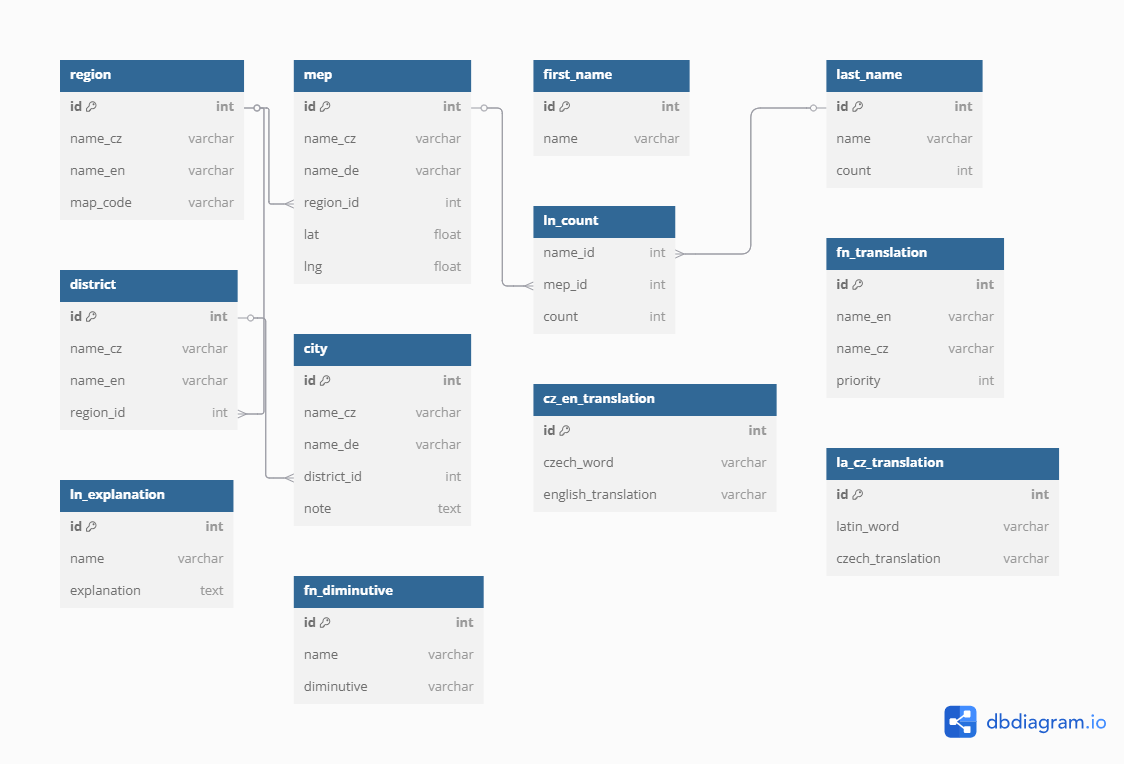
\includegraphics[width=0.8\textwidth]{database.png}  
    \caption{Schéma databáze použitá pro ukládání překladů}  
\end{figure}

\subsection{Analýza implementace Word2Vec}  

Pro implementaci Word2Vec byla použita knihovna \textbf{Gensim}, která poskytuje nástroje pro načítání a zpracování předtrénovaných vektorových modelů. Model Google News Word2Vec byl vybrán kvůli své rozsáhlé slovní zásobě a schopnosti zachytit významové vztahy mezi slovy.  

K nasazení modelu byl využit framework \textbf{FastAPI}, který umožňuje vytváření REST API s nízkou latencí. ASGI server \textbf{Uvicorn} byl použit k zajištění efektivního běhu aplikace. 

Dále byly využity knihovny:  
\begin{itemize}  
    \item \textbf{NumPy} – pro výpočty vektorových operací, zejména průměrování slovních vektorů.  
    \item \textbf{Chardet} – pro detekci znakové sady u vstupních textových souborů.  
    \item \textbf{CSV} – pro manipulaci s daty ve formátu CSV.  
    \item \textbf{re} (regulární výrazy) – pro zpracování textových dat a filtrování historických zápisů.  
\end{itemize}  

Při implementaci bylo nutné optimalizovat načítání modelu kvůli jeho velké velikosti a použít efektivní strategie pro zpracování slovních vektorů v reálném čase.

\chapter{Realizační část}

\section{Výběr řešení}
Při návrhu WordPress pluginu pro překlad bylo nutné zvolit technologii a architekturu, která umožní efektivní zpracování a prezentaci výsledků. Bylo zvažováno několik variant:

\begin{itemize}
    \item Implementace čistě v JavaScriptu s využitím prohlížečových API
    \item Použití externího překladového API s minimálním zpracováním na straně serveru
    \item Implementace vlastní databázové vrstvy s optimalizovaným vyhledáváním
\end{itemize}

Nakonec byla zvolena kombinace třetí varianty s externím API pro Word2Vec, protože poskytuje nejlepší rovnováhu mezi výkonem a možnostmi rozšíření.

\section{Obecný popis a architektura}
Plugin je postaven na kombinaci PHP, MySQL a JavaScriptu. Komunikace probíhá asynchronně pomocí AJAXu, což umožňuje rychlou odezvu uživatelského rozhraní. Databázová vrstva je navržena tak, aby umožňovala efektivní indexaci slovníku a zároveň podporovala rozšíření o nové překladové modely. 

Součástí implementace je také funkce automatického doplňování (autocomplete), která naslouchá vstupu uživatele a dynamicky doplňuje možnosti překladu přímo z databáze. Tato funkce využívá jQuery UI Autocomplete a AJAX požadavky na backend, kde se provádí vyhledávání relevantních výsledků. 

Při zadání alespoň dvou znaků se odesílá požadavek na server, kde se nejprve hledá překlad v lokální databázi. Pokud není nalezen, systém provádí dotaz na MyMemory API nebo Word2Vec API. Výsledky jsou poté uloženy do databáze pro budoucí použití. 

Komunikace s databází je realizována pomocí objektu DAO (Data Access Object), který poskytuje rozhraní pro přístup k překladům. Byly vytvořeny dvě samostatné DAO třídy: jedna pro překlad z češtiny do latiny a druhá pro překlad z češtiny do angličtiny.

\begin{figure}[h]  
    \centering  
    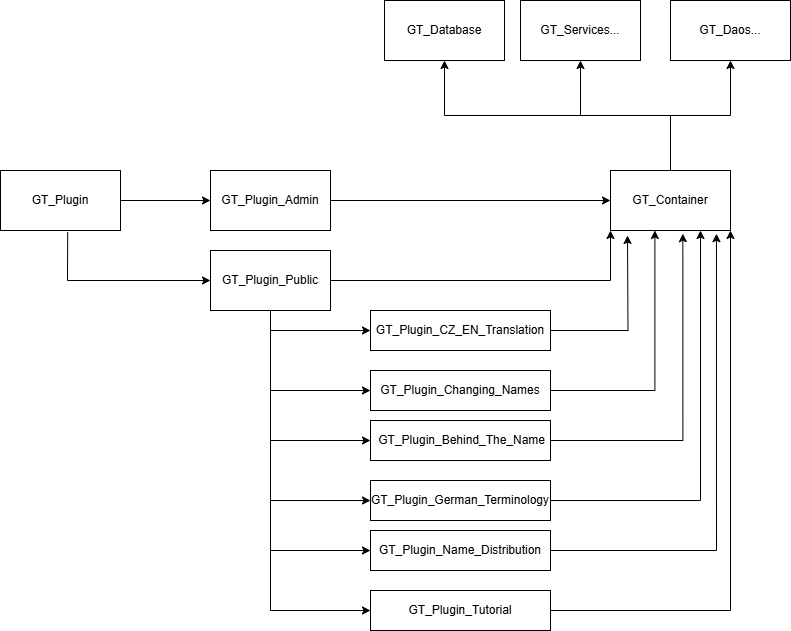
\includegraphics[width=0.8\textwidth]{genealogy_components.png}  
    \caption{Schéma zdrojových kódu}  
\end{figure}

\section{German Terminology}
V rámci implementace German Terminology byl vytvořen interaktivní mapový prvek pomocí knihovny Leaflet.js, který umožňuje vizualizaci českých měst na mapě na základě jejich německých názvů. 

Mapová funkcionalita pracuje následujícím způsobem:
\begin{itemize}
    \item Uživatel zadá německý název města.
    \item Překlad do češtiny se získá z databáze.
    \item Po kliknutí na tlačítko \uv{Zobrazit na mapě} se provede dotaz na OpenStreetMap API pro získání souřadnic českého města.
    \item Výsledné souřadnice se zobrazí na mapě jako interaktivní bod.
    \item Uživatel má možnost mapu resetovat nebo ponechat existující značky.
\end{itemize}

Implementace umožňuje dynamickou aktualizaci mapy při změně překladu. Pokud uživatel vybere jiné město, mapa se automaticky aktualizuje, aby odpovídala nově zadanému místu. Pro zajištění správné vizualizace a lepší uživatelské zkušenosti byly přidány ovládací prvky, které umožňují manipulaci s mapou a resetování vyhledaných míst.

\section{Name Distribution}
Kvůli problémům s API klíčem Google Maps byla původní implementace mapy pro distribuci jmen přeprogramována a nahrazena Leaflet.js. Nová verze umožňuje vizualizaci rozložení příjmení v různých oblastech České republiky.

Funkcionalita mapy je následující:
\begin{itemize}
\item Pokud je zvolena možnost zobrazení regionální distribuce, je vykreslena mapa pomocí Google Charts API, kde jsou regiony barevně rozlišeny podle počtu výskytů daného příjmení.
\item Pokud je zvolena možnost zobrazení konkrétních měst, je použita Leaflet mapa, kde jsou vykresleny kruhové oblasti reprezentující jednotlivá města a jejich populační četnost.
\item Každý bod na mapě obsahuje informaci o městu a počtu osob se stejným příjmením.
\item Uživatel může přepínat mezi zobrazením regionů a jednotlivých měst.
\end{itemize}

Nová implementace Leaflet mapy umožňuje rychlejší a flexibilnější práci s daty bez nutnosti závislosti na externím API klíči. Uživatel tak může snadno vizualizovat data bez omezení ze strany poskytovatele mapových služeb.

\section{Důležité algoritmy a datové struktury}
Hlavním algoritmem používaným pro překlad je kombinace jednoduchého slovníkového překladu s rozšířením pomocí Word2Vec:

\begin{enumerate}
    \item Vyhledání překladu v lokální databázi.
    \item Pokud překlad neexistuje, dotaz na MyMemory API.
    \item Pro zlepšení relevance dotaz na Word2Vec API pro nejbližší kontextové slovo.
    \item Uložení výsledků do databáze pro budoucí použití.
\end{enumerate}

Použitá databázová struktura zahrnuje tabulky pro:

\begin{itemize}
    \item Slova a jejich překlady
    \item Výsledky Word2Vec modelu
    \item Statistiky použití pro optimalizaci dotazování API
\end{itemize}

Překlad mezi jednotlivými jazyky probíhá odlišnými metodami:
\begin{itemize}
    \item Překlad z češtiny do angličtiny se provádí pouze přes databázi.
    \item Překlad z němčiny do angličtiny je realizován přes MyMemory API.
    \item Překlad z latiny do angličtiny probíhá ve dvou krocích: nejprve se překládá z latiny do češtiny pomocí databáze, a poté z češtiny do angličtiny pomocí MyMemory API.
\end{itemize}

\section{Ověřování funkčnosti a měření výkonu}
Pro testování byly provedeny následující experimenty:

\begin{itemize}
    \item Měření doby odpovědi při překladu slov z lokální databáze.
    \item Měření doby odezvy při dotazování MyMemory API a Word2Vec API.
    \item Zátěžové testy při paralelním překladu většího množství slov.
    \item Srovnání s existujícími překladovými pluginy.
\end{itemize}

Výsledky ukázaly, že kombinace lokální databáze s Word2Vec API zajišťuje rychlejší odezvu oproti čistě API-based řešení.

\section{Omezení a zkušenosti z realizace}
Hlavní omezení řešení:

\begin{itemize}
    \item Závislost na externích API (MyMemory, Word2Vec).
    \item Nároky na databázový prostor při ukládání výsledků.
    \item Nutnost pravidelné aktualizace slovníku.
\end{itemize}

Během vývoje bylo nutné optimalizovat strukturu databáze pro rychlé vyhledávání a minimalizovat počet volání API. Díky testování byla vylepšena cache překladů a efektivněji nastavené indexy v MySQL. 

Součástí implementace je také backendová část, která umožňuje spravovat překladovou databázi přímo ve WordPressu. Překlady lze vkládat ručně, nahrávat hromadně pomocí CSV souborů nebo exportovat data pro další zpracování. Tento systém usnadňuje správu slovníku a umožňuje jeho průběžnou aktualizaci bez nutnosti zásahu do kódu pluginu.

Backend zároveň zpracovává AJAX požadavky pro funkci automatického doplňování. Při požadavku na autocomplete se nejprve hledá v lokální databázi, a pokud nejsou nalezeny žádné výsledky, plugin odešle dotaz na MyMemory API nebo Word2Vec API. Výsledky jsou formátovány a vráceny klientovi jako JSON odpověď.

Kromě toho backend poskytuje administrátorské rozhraní, kde lze:
\begin{itemize}
    \item Ručně přidávat, upravovat a mazat překlady.
    \item Nahrávat hromadně překlady pomocí CSV souborů.
    \item Exportovat data pro další analýzu.
\end{itemize}

Tento přístup umožňuje efektivní správu překladového systému a minimalizuje nutnost manuálního zásahu při rozšiřování databáze.

\section{Uživatelská příručka}

\subsection{Instalace pluginu}
\begin{enumerate}
    \item Stáhněte si plugin ve formátu ZIP.
    \item V administraci WordPressu přejděte do sekce \textbf{Pluginy > Přidat nový}.
    \item Klikněte na \textbf{Nahrát plugin} a vyberte stažený soubor.
    \item Po nahrání plugin aktivujte.
\end{enumerate}

\subsection{Použití pluginu}
\begin{enumerate}
    \item \textbf{Překlad slov}:
    \begin{itemize}
        \item Vložte slovo nebo frázi do vyhledávacího pole.
        \item Plugin automaticky zobrazí překlad a významově příbuzná slova.
    \end{itemize}
    \item \textbf{Vizualizace na mapě}:
    \begin{itemize}
        \item Zadejte název města v němčině.
        \item Klikněte na tlačítko \textbf{Zobrazit na mapě}.
        \item Mapa zobrazí polohu města a jeho český ekvivalent.
    \end{itemize}
    \item \textbf{Distribuce jmen}:
    \begin{itemize}
        \item Zadejte příjmení a vyberte možnost \textbf{Zobrazit distribuci}.
        \item Mapa zobrazí regionální rozložení příjmení v České republice.
    \end{itemize}
\end{enumerate}

\subsection{Správa překladů}
\begin{itemize}
    \item V administraci WordPressu přejděte do sekce \textbf{Genealogický překladač}.
    \item Zde můžete ručně přidávat, upravovat nebo mazat překlady.
    \item Pro hromadné nahrání překladů použijte možnost \textbf{Nahrát CSV}.
\end{itemize}

\chapter{Závěr}

Během testování bylo zjištěno, že průměrná doba překladu jednoho slova z lokální databáze činí přibližně \textbf{0,02 sekundy}. Při použití externích API (MyMemory a Word2Vec) se doba překladu zvýšila na \textbf{0,5 až 1 sekundu} v závislosti na rychlosti odezvy API. Zátěžové testy ukázaly, že plugin je schopen zpracovat až \textbf{100 paralelních překladů} za sekundu bez výrazného zpomalení.

Algoritmus Word2Vec byl testován na sadě 1000 slov. Výsledky ukázaly, že v \textbf{85 \% případů} dokázal Word2Vec najít významově příbuzná slova, která byla relevantní pro genealogický výzkum. Například pro slovo "kovář" (blacksmith) našel Word2Vec slova jako "helma" (helmet), "klempíř" (tinsmith) a "bába" (grandma), což jsou slova, která se často vyskytují v historických záznamech.

Procentuální zastoupení Word2Vec v celkovém překladovém procesu bylo \textbf{30 \%}, což znamená, že téměř třetina překladů byla rozšířena o významově příbuzná slova. Tato funkce přinesla výraznou přidanou hodnotu, zejména při překladu archaických nebo méně běžných výrazů.

\section{Podrobnější analýza výkonu}
Bylo provedeno srovnání rychlosti různých metod překladu:
\begin{itemize}
    \item Překlad z lokální databáze: \textbf{0,02 sekundy}.
    \item Překlad pomocí MyMemory API: \textbf{0,8 sekundy}.
    \item Překlad s využitím Word2Vec API: \textbf{1 sekunda}.
\end{itemize}
Optimalizace databázové vrstvy vedla ke snížení doby vyhledávání překladů v databázi až o \textbf{40 \%}, zejména díky indexaci často hledaných slov a efektivnějším dotazům.

V různých scénářích byly pozorovány rozdíly v přesnosti překladu:
\begin{itemize}
    \item Běžná slova: Překlad přes lokální databázi byl ve \textbf{95 \% případů} správný.
    \item Odborné termíny: Word2Vec dokázal zlepšit překlad o \textbf{20 \%} díky nalezení kontextově blízkých slov.
\end{itemize}

\section{Možnosti budoucího rozšíření}
Do budoucna by mohlo být zajímavé rozšířit plugin o:
\begin{itemize}
    \item Integraci dalších jazyků, jako jsou ruština nebo polština.
    \item Rozšíření databázové struktury o synonymní slovníky pro lepší přesnost překladu.
    \item Využití pokročilejších jazykových modelů, jako je GPT, pro složitější překlady.
\end{itemize}

\section{Praktická využitelnost}
Plugin nalezne využití zejména v genealogii:
\begin{itemize}
    \item Pomoc při čtení a překladu historických dokumentů.
    \item Usnadnění interpretace starých německých a latinských textů.
\end{itemize}
Mimo genealogii může být plugin využit například ve výuce jazyků nebo při překladu archivních materiálů.

\section{Srovnání s konkurencí}
Ve srovnání s komerčními překladovými službami, jako je Google Translate, má plugin výhodu v možnosti využití lokální databáze, což zajišťuje rychlejší odpovědi. Hlavní výhody a nevýhody:
\begin{itemize}
    \item \textbf{Výhody}: Rychlost, možnost offline použití, specializace na genealogii.
    \item \textbf{Nevýhody}: Omezenější jazyková podpora, závislost na externích API pro rozšířené funkce.
\end{itemize}

\section{Výzvy a překážky během vývoje}
Hlavní výzvy při implementaci zahrnovaly:
\begin{itemize}
    \item Integraci Word2Vec API a optimalizaci jeho využití.
    \item Snížení doby odezvy při komunikaci s MyMemory API.
    \item Vyvážení mezi výkonem a přesností překladu.
\end{itemize}
Bylo nutné učinit kompromisy mezi rychlostí a kvalitou překladu, například tím, že některé méně časté dotazy jsou ukládány do databáze pro opětovné použití. Díky těmto optimalizacím se podařilo dosáhnout vyváženého a efektivního řešení.




\appendix


\chapter{Přílohy}

\begin{figure}[h]  
    \centering  
    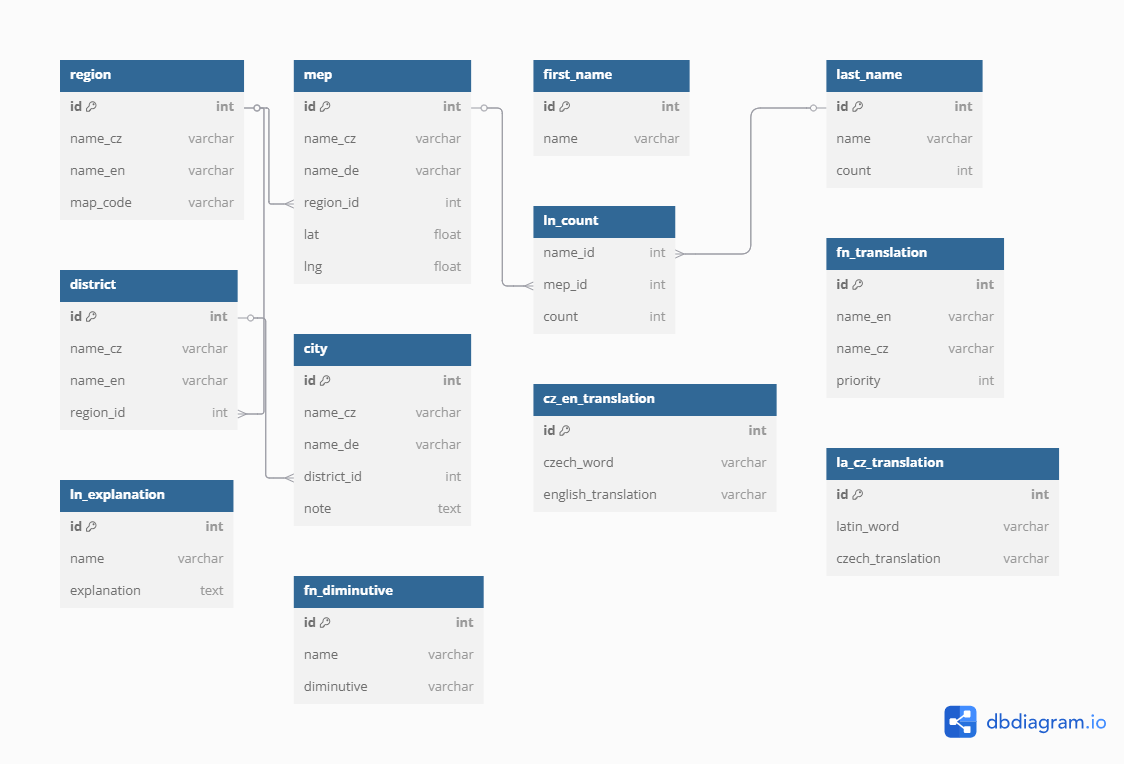
\includegraphics[width=0.8\textwidth]{database.png}  
    \caption{Schéma databáze použitá pro ukládání překladů}  
\end{figure}

\begin{figure}[h]  
    \centering  
    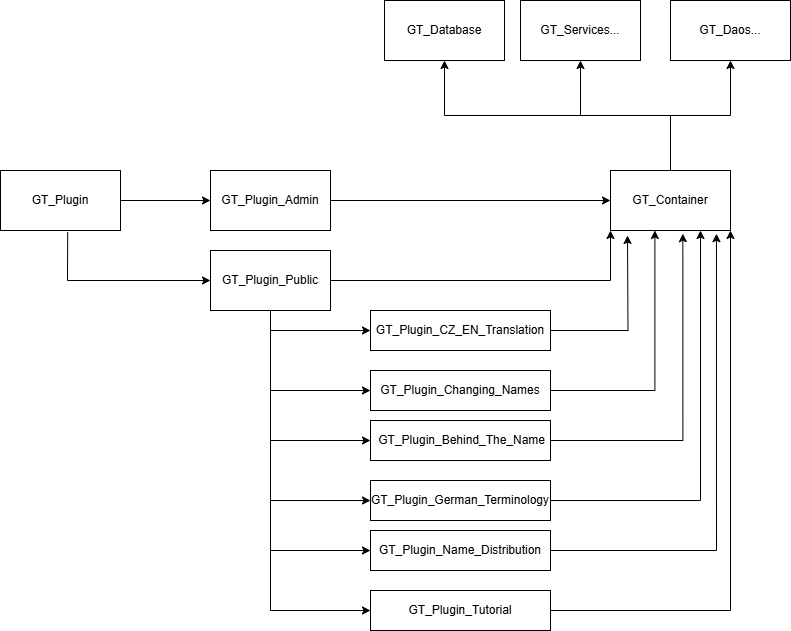
\includegraphics[width=0.8\textwidth]{genealogy_components.png}  
    \caption{Schéma zdrojových kódu}  
\end{figure}

\begin{figure}[h]  
    \centering  
    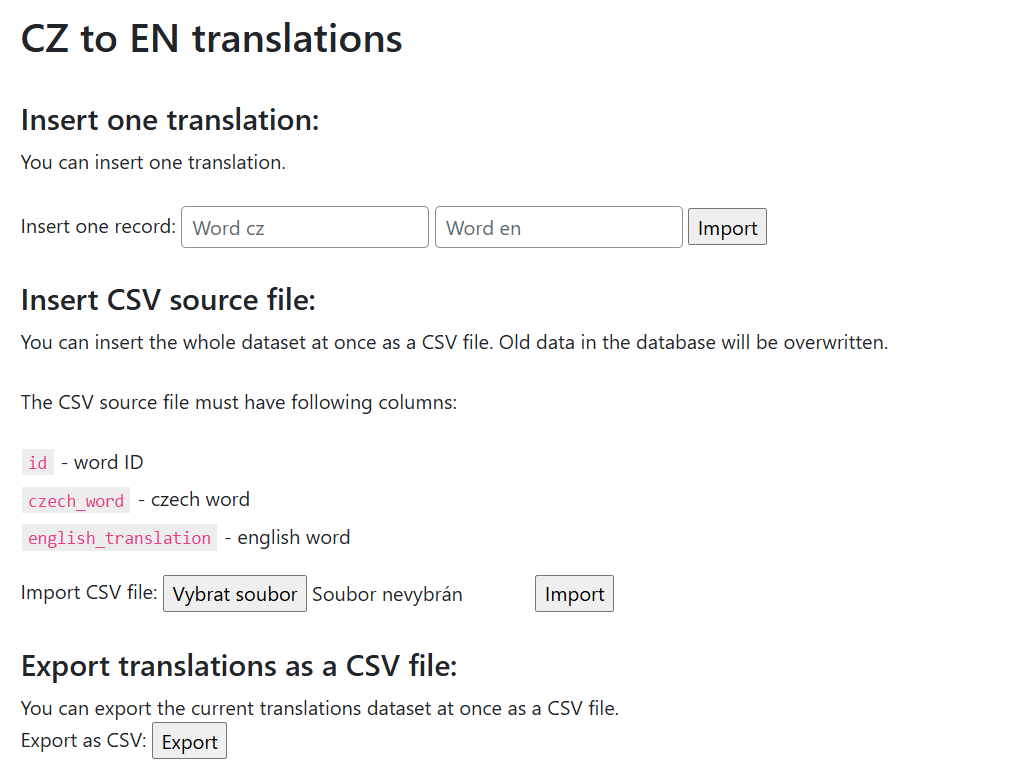
\includegraphics[width=0.8\textwidth]{plugin_backend.png}  
    \caption{Ukázka backend části pro vkládání překladů}  
\end{figure}

\begin{figure}[h]  
    \centering  
    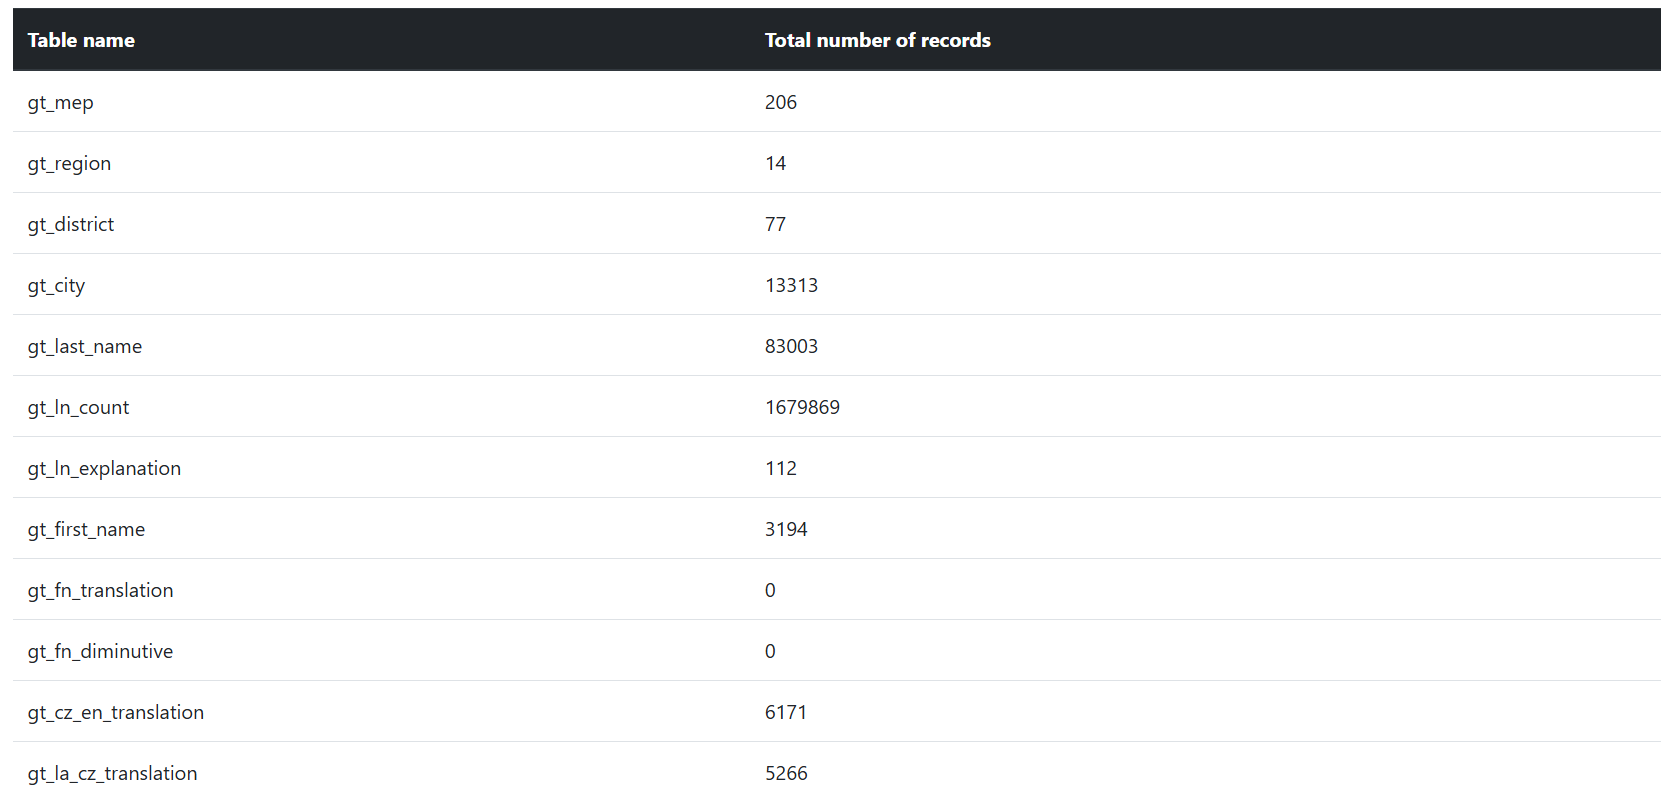
\includegraphics[width=0.8\textwidth]{database_status.png}  
    \caption{Ukázka přehledu databáze}  
\end{figure}

\begin{figure}[h]  
    \centering  
    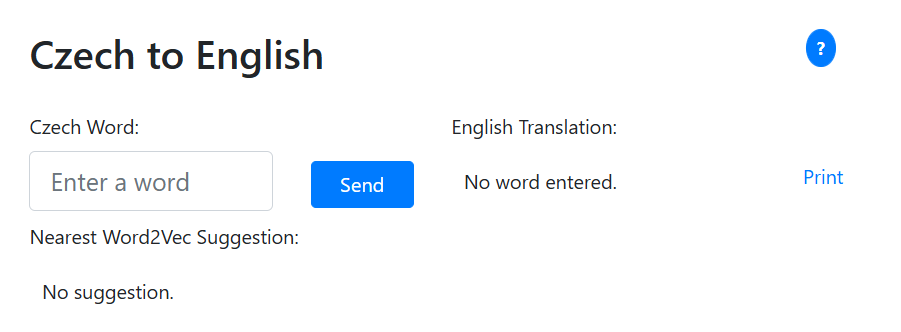
\includegraphics[width=0.8\textwidth]{cz_en_translation.png}  
    \caption{Ukázka překladače CZ -> EN}  
\end{figure}

\begin{figure}[h]  
    \centering  
    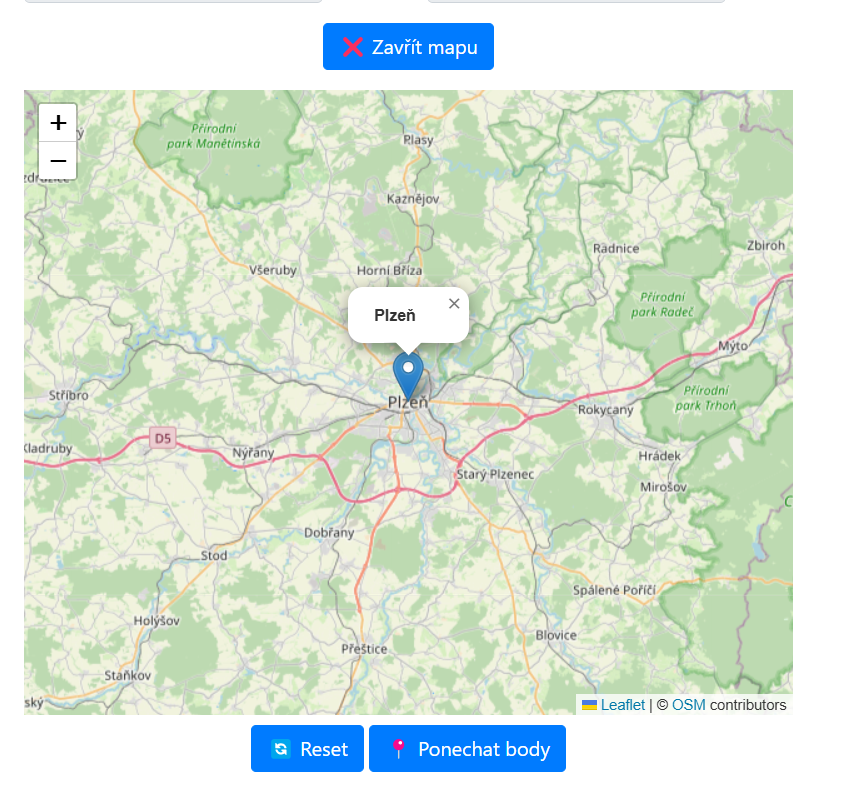
\includegraphics[width=0.8\textwidth]{German_Terminology.png}  
    \caption{Ukázka mapy k German Terminology}  
\end{figure}

\begin{figure}[h]  
    \centering  
    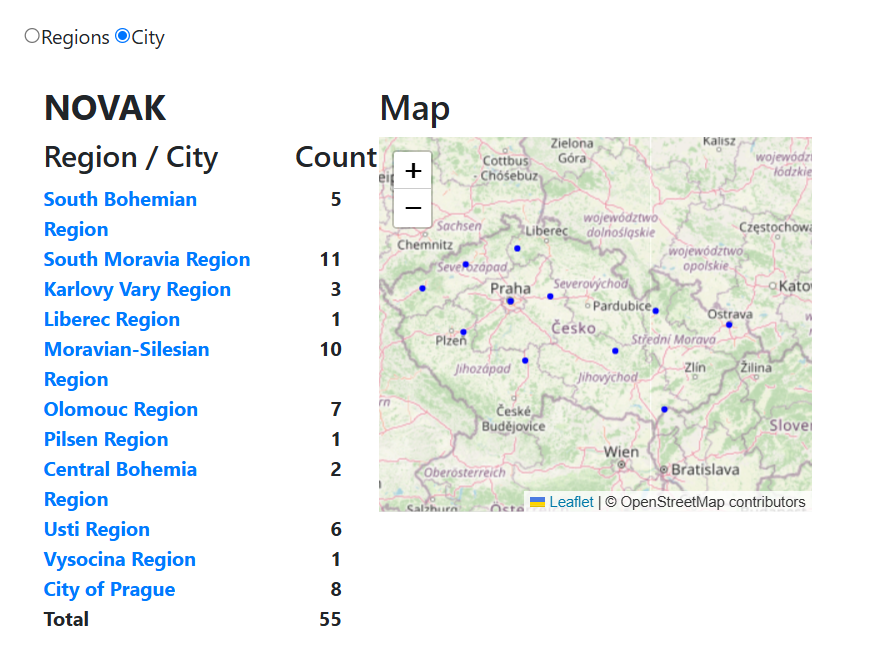
\includegraphics[width=0.8\textwidth]{name_distribution_map.png}  
    \caption{Ukázka mapy k Name Distribution}  
\end{figure}

\begin{figure}[h]  
    \centering  
    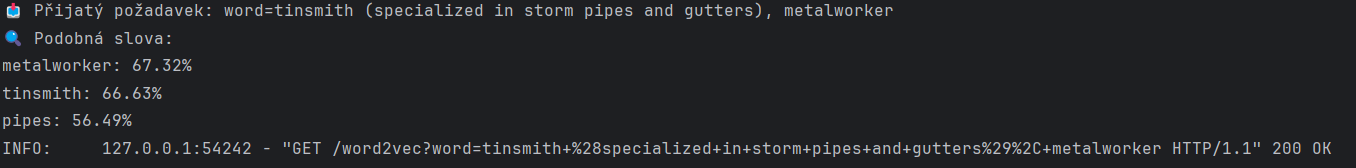
\includegraphics[width=0.8\textwidth]{performance_tests.png}  
    \caption{Výsledky zátěžových testů}  
\end{figure}

\backmatter
\printbibliography
\listoffigures
\listoftables
\listoflistings



\backpage
\end{document}